\documentclass[14pt]{report}
\usepackage[utf8]{inputenc}
\usepackage{amsmath} % for using & and align formulas
\usepackage{parskip} % new paragraph adds a blank line before
\setlength{\parindent}{0in} % no indent
\renewcommand{\familydefault}{\sfdefault} %change font to ss
\usepackage{graphicx} %include images
\graphicspath{{images/}}
\usepackage{fancyvrb}
\usepackage{hyperref} %for links on labels and table of contents

\begin{document}
\tableofcontents
\chapter{Introduction to neural networks}
\section{High Level View}

On its core, Machine Learning about is a program that changes from exposure to data (experience).

Normally, data and parameters are the input to the model (mathematical function). This outputs a prediction, that we use to update the parameters in such a way that it better fits the data.

Deep Learning models complex patterns of data. It's particularly useful for non-linear patterns. This opens up a new space of problems to solve. Because Deep Learning is a part of Machine Learning, the previous logic is found neural network diagrams.

Network Diagrams can be found in section \ref{section:figs} 

\section{The steps}
There are two main steps: \textit{forward} and \textit{backward} propagation. 

Suppose a mathematical function is given to us:
$$ \hat{y}(x_1,x_2) = a x_1 + b x_2 + c$$
where $a$, $b$, $c$ are \textit{parameters}.

In \textbf{Forward Propagation} we initialize a set of parameters (say $a,b,c=0$), and use the equation to estimate the real output ($y$). Both values are input to ``$C(y, \hat{y})$'' which is small if we're doing well, or large if bad. 

So forward propagation is the calculation of $\hat{y}$ and $C(y,\hat{y})$ whatever shape they happen to have. 

In the next chapters $y$, $\hat{y}$ are $a$ and $\hat{a}$; this is just the notation used in ML/DL.

In \textbf{Backward Propagation} we minimize $C$, by differentiation, and find a way to move our function parameters towards the minimum of $C$. We use \textit{Gradient Descent} for this task.

The simplest neural network is the single layer. Later, hidden layers are included, from 1 (shallow network), to many (deep network).

We will see examples in detail, starting with multivariable linear regression, that is, a previous step to \textit{Deep Learning}.

\section{Summary}
Calculate $\hat{y}$ which is an estimation of $y$, compute $C(y,\hat{y})$, and use this to update $\hat{y}$ parameters, iteratively.

\section{Figures}\label{section:figs}
\begin{figure}[h]
 \centering
 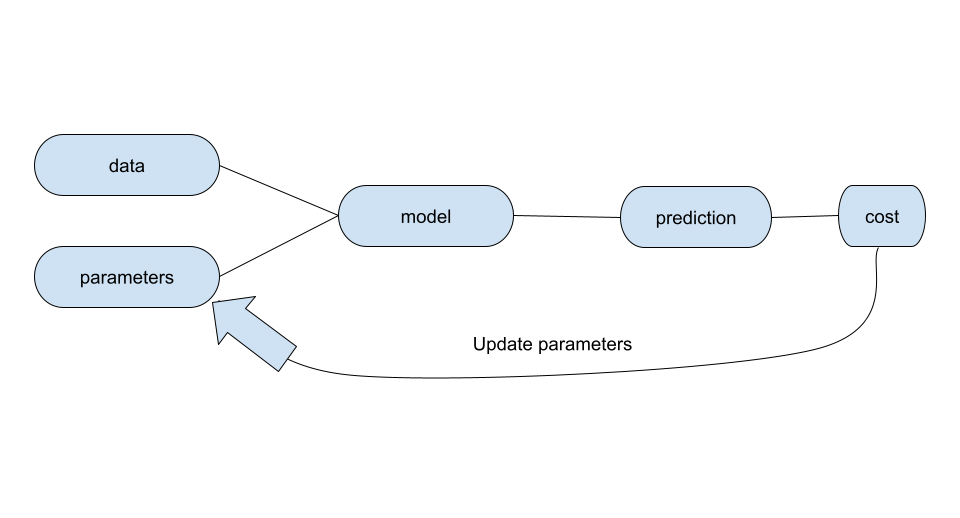
\includegraphics[width=0.9\textwidth]{ml.png}
  \caption{Machine Learning Process}\label{fig:learn}
\end{figure}

\begin{figure}
 \centering
 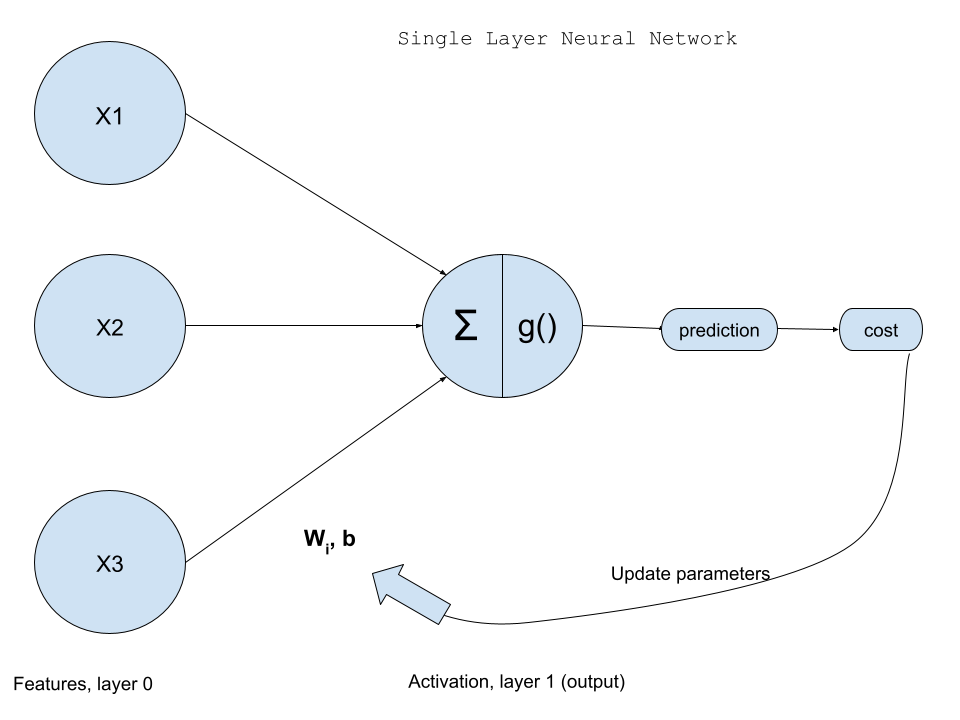
\includegraphics[width=\textwidth]{1L-NN.png}
 \caption{Single Layer Neural Network}
 \label{fig:single}
\end{figure}

\begin{figure}
 \centering
 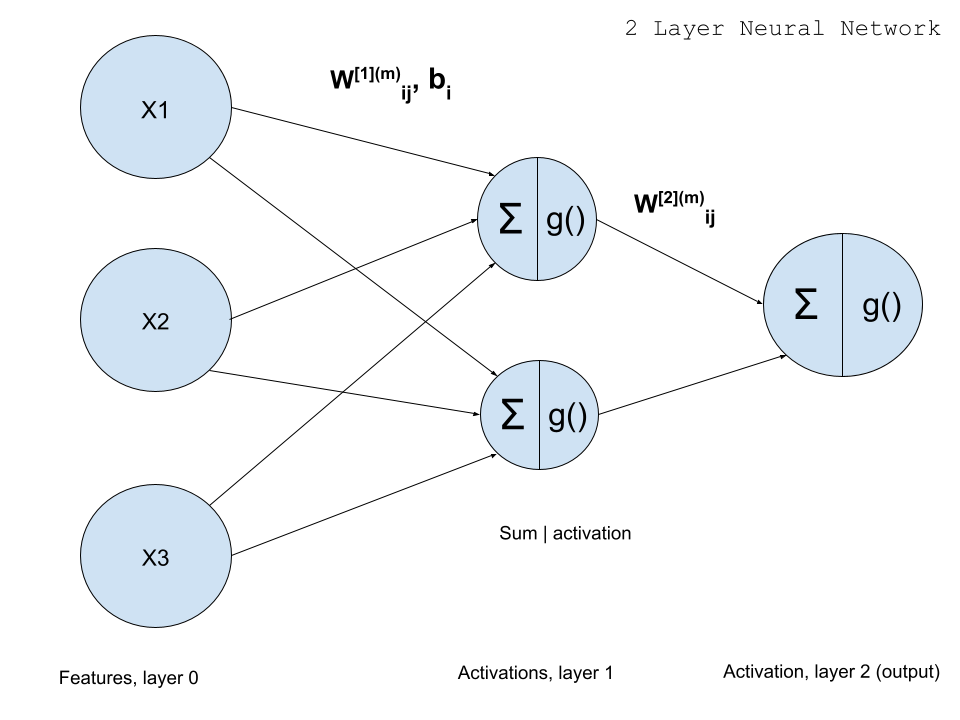
\includegraphics[width=\textwidth]{2L-NN.png}
 \caption{Shallow Neural Network}
 \label{fig:shallow}
\end{figure}

\section{Example: Multivariable Linear Regression}
A linear regression model for 2 features:
\begin{align*}
  a(x_1, x_2) &= w_1\,x_1 + w_2\,x_2 + b \\
   &= \vec{w}\cdot\vec{x} + b
\end{align*}
$w_1$,$w_2$ control the slopes of this plane, $b$ translates it up and down. $\vec{x}$ is for one sample. Two or more samples are represented as a matrix:
\begin{align*}
[a_1, a_2] = 
  [w_1, w_2]\cdot{}
  \begin{bmatrix}
  x_1 & x_1\\
  x_2 & x_2 
  \end{bmatrix}
 +  b
\end{align*}
$a_i$ is the result for each sample (columns in the matrix).

The same than for a line (figure \ref{fig:line}) by tuning $W$ and $b$  we can find the best linear fit. The sign of $W$ reflects the line over Y($a$) axis, and its magnitude controls the slope; $b$ translates the line over $x$. Without $b$ the line has to go through the origin. 

We need to do forward and backward propagation.
\begin{figure}[h]
 \centering
 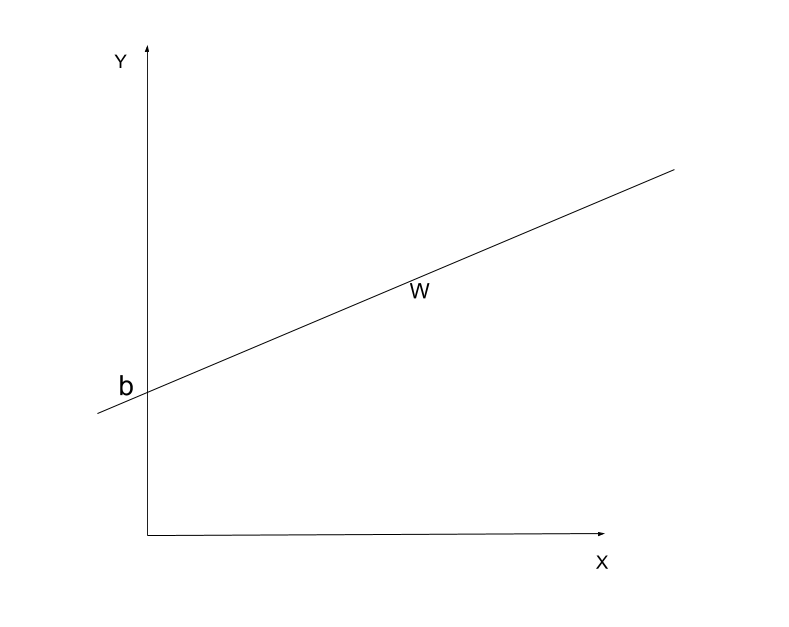
\includegraphics[width=0.9\textwidth]{line_plot.png}
  \caption{Line plot} \label{fig:line}
\end{figure}


\subsection{Forward Propagation}
The Loss denoted $= Loss(w_1,\ldots, w_n, b)$ or just $L(\vec{w},b)$ in linear regression is the \textit{Square Error}:
\begin{align*}
  L_i(\vec{w}, b) &= (a_i - \hat{a})^2\\
  &=(a_i -\vec{w}\cdot{}\vec{x}_{i} -b)^2
\end{align*}
$\vec{w}\cdot{}\vec{x}_i$ can also be denoted $\sum_jw_j\cdot{}\mathbf{X}_{ji}$. In the first form we multiply the vector $w$ and the column $i$ (dot product).

In Linear Regression, the Cost is the averaged sum of $L_i$, and it's the \textit{Mean Square Error}:
\begin{align}
  C(w_1, w_2, b) &= \frac{1}{2} \sum_{i=0}^{i=2} L_i(w_1, w_2, b)\nonumber\\
  &= \frac{1}{2}([a_1, a_2] - [\hat{a}_1, \hat{a}_2])\cdot{}([a_1, a_2]-[\hat{a}_1, \hat{a}_2])\nonumber\\
  &=\frac{1}{2}([a_1, a_2] - [w_1, w_2]\cdot{}\mathbf{X}-b)\cdot{}([a_1, a_2] - [w_1,w_2]\cdot{}\mathbf{X} -b) \label{cost}
\end{align}
$\frac{1}{2}$ is to average over examples. Equation \ref{cost} is what we implement into code.
%Outliers may be critical on the effect of weights and biases.

In Python it'd look like:
\begin{center}
  \begin{BVerbatim}
  Ap = np.dot(w,X) - b
  diff = A-Ap 
  cost = 1/2*np.dot(diff, diff.T)
  \end{BVerbatim}
\end{center}





\subsection{Backward Propagation}
\begin{figure}
  \centering
  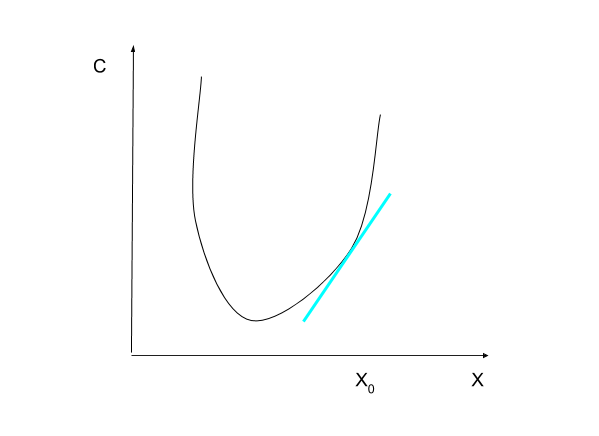
\includegraphics[width=0.75\textwidth]{derivative.png}
  \caption{Derivative}\label{fig:basics}
\end{figure}

For a function of a single variable $C(x)$ the derivative at a point $x_0$ is the slope (figure \ref{fig:basics}) at $x_0$.

For many variables, it's a similar process: the total derivative of a function is the sum of partial derivatives.

\begin{align}
  dC(\vec{w},b) &= \frac{\partial C}{\partial w_1}+ \frac{\partial C}{\partial w_2} + \frac{\partial C}{\partial b}\\
\end{align}
$C(w,b)$ derivative is used to find better weights and bias:
\begin{align*}
  \vec{w} &= [w_1, w_2] - [\frac{\partial C}{\partial w_1},\frac{\partial C}{\partial w_2}]\cdot{}\alpha\\
  \vec{w} &= \vec{w} -\frac{\partial C}{\partial \vec{w}}\cdot{}\alpha\\
  b &= b -\frac{\partial C}{\partial b}\cdot{}\alpha
\end{align*}
Let's get started.
\begin{align}
  dC(\vec{w},b) &= \frac{\partial C}{\partial w_1}+ \frac{\partial C}{\partial w_2} + \frac{\partial C}{\partial b}\\
  &= d(\sum_{i=0}^{i=2}L_i) = \sum_{i=0}^{i=2}dL_i(\vec{w},b) \label{diffp}\\
  &=\sum_{i=0}^{i=2} \frac{\partial L_i}{\partial w_1} +\frac{\partial L_i}{\partial w_2} + \frac{\partial L}{\partial b}
\end{align} 
These equations are important. Equation \ref{diffp} makes use of linearity property of diff.

We sum over columns (each sample). Now, pick up a column/sample $k$:
\begin{align*}
  L_k(\vec{w},b) &= (a_k - \hat{a}_k)^2\\
    L_k &= A_k(w_1, w_2, b)^2\\
    dL_k &= 2\,A_k(w1,w2,b)\,dA_k
\end{align*}
$A_k$ is the difference $a_k-\hat{a}_k$. We need $dw$ and $db$; and for this $dA_k$:
\begin{align*}
  dL_k  &= 2A_k\,(\frac{\partial A_k}{\partial w_1} + \frac{\partial A_k}{\partial w_2} + \frac{\partial A_k}{\partial b}) \\
  A_k &= A_k(w_1, w_2, b)\\
  &= a_k - \vec{w}\cdot{}\vec{x_k} - b\\
  &= a_k - w_1\,x_{1k} - w_2\,x_{2k}-b\\
  dA_k &= -x_{1k} - x_{2k} -1
\end{align*}
where 
\begin{center}
\begin{align*}
  \frac{\partial A_{k}}{\partial w_1} = -x_{1k}\hspace{2em} \frac{\partial A_{k}}{\partial w_2} = -x_{2k}\hspace{2em} \frac{\partial A_k}{\partial b} = -1
\end{align*} 
\end{center}

This can be expressed in compact form:
\begin{align*}
  dC &= sum(-\frac{1}{2}\times{}2\mathbf{X}\cdot{}\vec{A^T}-\frac{1}{2}\times{}2\vec{A}\times{}\vec{1})\\
  &= \frac{\partial C}{\partial \vec{w}} + \frac{\partial C}{\partial b} 
\end{align*}

To update the parameters, \textit{Gradient Descent} method is used. We update the vector $\vec{w}$ as follows:
\begin{align}
  \vec{w} &= \vec{w} -\frac{\partial C}{\partial \vec{w}}\cdot{}\alpha\\
  b &= b -\frac{\partial C}{\partial b}\cdot{}\alpha
\end{align}
$\alpha$ is called \textit{learning rate} and we use to tune the derivation. We go against the gradient so the sign is changed to $-$ (it points to max incresing direction otherwise).

In deep neural networks $b$ will explicitly be a vector.

\subsubsection{Interpretation}

There is no graphical justification as to why we update $w$ and $b$ like that, but we are moving $w$ against (minus) the gradient multiplied by a constant (alpha) called \textit{learning rate}.

The minus sign is because the gradient always points away from the minimum and we want towards it (in one dimension there are only 2 directions). 

\begin{align}
  \vec{w} &= \vec{w} -\frac{\partial C}{\partial \vec{w}}\,\alpha\\
  &= \vec{w} -[\frac{\partial C}{\partial w_1}, \frac{\partial C}{\partial w_2},\ldots, \frac{\partial C}{\partial w_n}]\,\alpha\\
\end{align}

It means we have a vector of corrections for each slope such that the overall cost is decreased. If we take say $\frac{dC}{dw1}$ it is the sum of slopes for each sample, divided by $m$. 

To have more insight and detail, we could take a look at a dataset with just one feature. Then 
\begin{align*}
  C &= \frac{1}{m}\sum_i(a_i - \hat{a}_i)^2 \\ 
  \frac{\partial C}{dw_1}&= \frac{1}{m}\,\sum_i \frac{dL_i}{dw_1} \\
  &= -\frac{2}{m}\sum_i \mathbf{X}_{1i}(\vec{a}_i-\vec{\hat{a}}_i)
\end{align*}
we see the slope depends on the sum of features times errors. Much more can be inspected here.

%This is almost the same result we get in the \textit{sigmoid}, just multiplied by $2$. Because the $2$ can be thought as inside the learning rate, we can use the exact same \textit{backpropagation} for both methods!

\section{Linear Regression: General Derivation}
Only main differences are shown as the process is the same.

The problem is to find $w_i$, $b$ such that the multidimensional ``plane'' has small error respect to each datapoint. Then for a new datapoint we will have a trained predictor.

In linear regression, the model is:
\begin{align*}
 a &= w_1\, x_1 + w_2\, x_2 +\ldots+ w_n\, x_n\\
   &= \sum_i^n w_i\, x_i + b \\
   &= \vec{w}\cdot\vec{x} + b
\end{align*}
Here $\vec{x}$ is for one sample. For $n$ samples, it becomes a matrix, we write $\vec{y} = \vec{w}\cdot\mathbf{X} + \vec{b}$. This is represented:
\begin{equation*}
  [a_1, a_2, \ldots, a_n] = 
  [w_1, w_2, \ldots, w_n] \cdot
  \begin{bmatrix}
    x_{11} & x_{12} & \ldots & x_{1m}\\
    x_{21} & x_{22} & \ldots & x_{2m}\\
    \vdots & \vdots & \ddots & \vdots\\
    x_{n1} & x_{22} & \ldots & x_{nm}\\
  \end{bmatrix}
  + [b_1, b_2, \ldots, b_m]
\end{equation*}
The $b_i$ are all the same number. There are $m$ examples-columns with $n$ features-rows. Hence $[\mathbf{X}] = m\times{}n$


\section{Sigmoid}
The derivation is similar to Linear regression. The plot for the equation:
\[
y = \frac{1}{1+e^{-(\vec{w}\cdot{}\vec{x}+b)}}
\]

for one dimension is on figure \ref{fig:sigmoid}. By tuning $W$ and $b$  we can find the best fit. 

The sign of $W$ reflects the line over $y$ axis, and the slope. Also $b$ translates over $x$.

\begin{figure}[h]
 \centering
 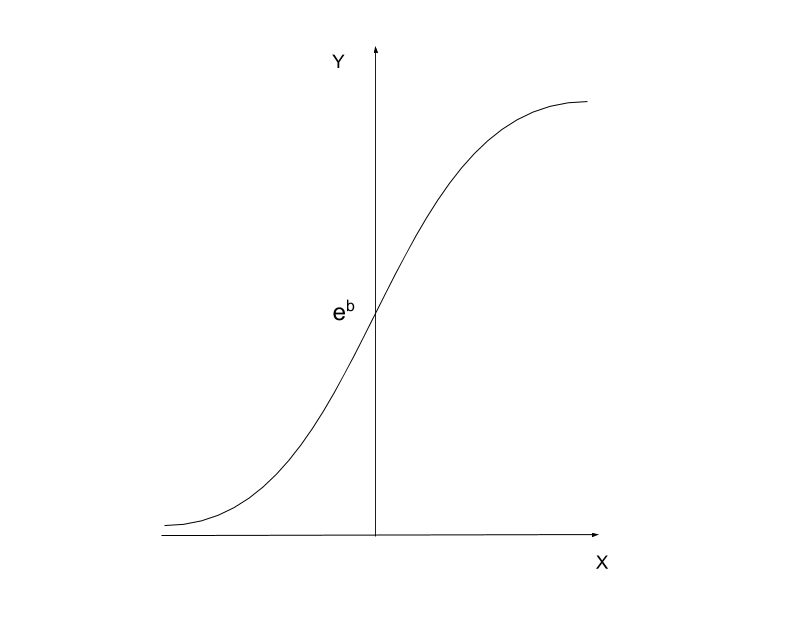
\includegraphics[width=0.9\textwidth]{sigmoid_plot.png}
  \caption{Sigmoid plot} \label{fig:sigmoid}
\end{figure}






\section{Results}
In general, non-normalized data blows up some calculation.
In sigmoid, it is the exponential $wX+b$; in linear, because of $A^2$ in the cost. Here also the learning rate can be really large (up to 100) and the code optimizes well. With smaller learning rates, we need more cycles.

The backward propagation ends up being the same for both methods (apart from a constant). Hence it is useful for both methods. The cost is different though.


\chapter{More complex networks}
\section{Multiclass Network}

This network can be used for multiclass problems, but it's actually used with a \textit{softmax} function instead of \textit{sigmoid}. 

Now the results and predictions are column vectors. The cost can be thought now as a row vector of $N$ components, for $N$ classes/labels.

From the NN diagram, we derive the computations:

\begin{equation*}
  \begin{bmatrix}
    a_{11} & a_{12}& \ldots& a_{1m}\\ 
    a_{12} & a_{22}& \ldots& a_{2m}\\ 
    \vdots & \vdots & \vdots& \vdots\\ 
    a_{s1} & a_{s2}& \ldots& a_{sm} 
  \end{bmatrix}
    =\sigma( 
  \begin{bmatrix}
    w_{11} & w_{12}& \ldots& w_{1n}\\ 
    w_{12} & w_{22}& \ldots& w_{2n}\\ 
    \vdots & \vdots & \vdots& \vdots\\ 
    w_{sn} & w_{sn}& \ldots& w_{sn} 
  \end{bmatrix}
  \cdot{}
  \begin{bmatrix}
    x_{11} & x_{12} & \ldots & x_{1m}\\
    x_{21} & x_{22} & \ldots & x_{2m}\\
    \vdots & \vdots & \ddots & \vdots\\
    x_{n1} & x_{22} & \ldots & x_{nm}\\
  \end{bmatrix}
  +
  \begin{bmatrix}
    b_1\\ b_2\\ \vdots\\ b_s
  \end{bmatrix})
\end{equation*}
$s$ dimension is equal to the number of nodes in the output layer, and $n$ to the number of features on the input layer. $\mathbf{B}$ will actually be broadcasted to match the shape of $\mathbf{A}$. 

The cost for the $j$ node is:
\begin{align}
  C_j = -\frac{1}{m}\left(\sum_i \mathbf{A}_{ji}\log(\hat{\mathbf{A}}_{ji}) + (1-\mathbf{A}_{ji})\log(1-\hat{\mathbf{A}}_{ji})\right) 
\end{align}
which may be coded like this:
\begin{verbatim}
C = np.sum(
         multiply(A, np.log(Ap))
       + multiply(1-A, np.log(1-Ap)),
       axis=0)
\end{verbatim}
The gradients are: 
\begin{align}
  \frac{dC}{d\mathbf{W}} &= \mathbf{X}\cdot{}\mathbf{\Delta A}^T\\
  \frac{dC}{d\mathbf{B}} &= \mathbf{\Delta A}
\end{align}

$\mathbf{A}$ was a vector, now it's turned into a matrix, one row for each node. Same thing for $\mathbf{W}$.

\section{Shallow Neural Network}

Standalone regressions approximate data with a single function. Hence they can't represent complex patterns. 

\begin{figure}
  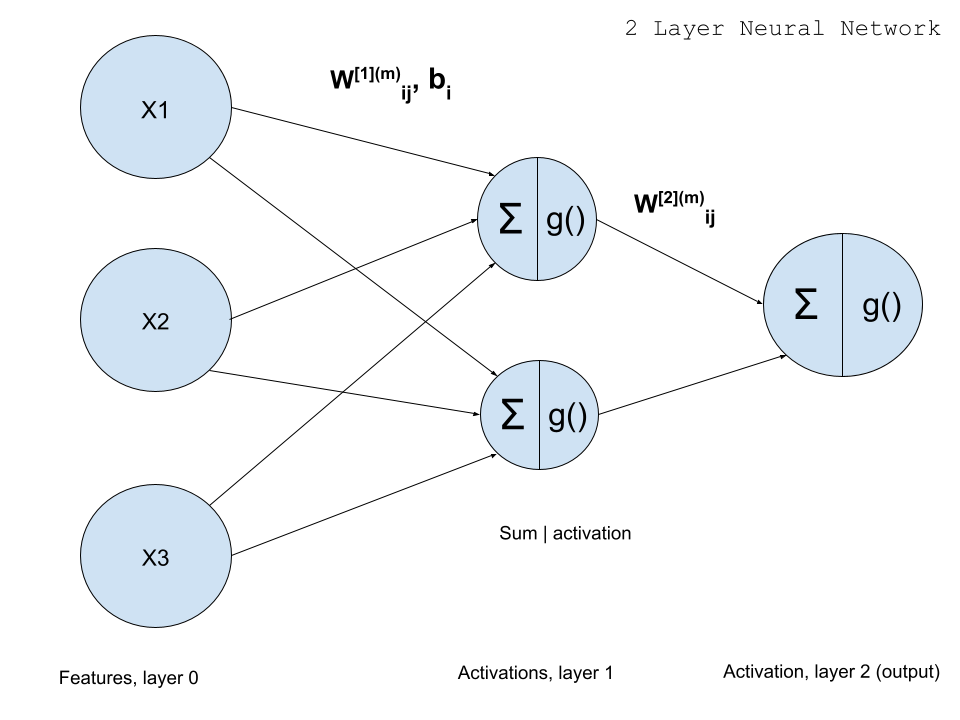
\includegraphics[width=\textwidth]{2L-NN.png}
  \caption{Shallow NN diagram}\label{fig:shallow}
\end{figure}
We calculate what is shown in \ref{fig:shallow}.

\subsection{Forward Propagation}
What changes is $W$, passes from a vector to a matrix. Each row will represent a node.

\begin{align}
  \mathbf{A} = \mathbf{W} \cdot{} \mathbf{X} + \mathbf{B} \label{eq:multi}
\end{align}

\begin{equation*}
  \begin{bmatrix}
    a_1^1 &\ldots & a_m^1\\
    a_1^2 &\ldots & a_m^2\\
    \vdots &\ldots & \vdots\\
    a_1^s &\ldots & a_m^s\\
  \end{bmatrix}
  = 
  \begin{bmatrix}
    w_1^1& w_2^1& \ldots& w_n^1\\
    w_1^2& w_2^2& \ldots& w_n^2\\
    \vdots& \vdots& \ddots& \vdots\\
    w_1^s& w_2^s& \ldots& w_n^1\\
  \end{bmatrix}
  \begin{bmatrix}
    x_{11} & x_{12} & \ldots & x_{1m}\\
    x_{21} & x_{22} & \ldots & x_{2m}\\
    \vdots & \vdots & \ddots & \vdots\\
    x_{n1} & x_{22} & \ldots & x_{nm}\\
  \end{bmatrix}
  + \begin{bmatrix}b_1\\ b_2\\ \vdots\\ b_n\end{bmatrix}
\end{equation*}

$A$ acts now like $X$, each column being a sample. Each row belongs to a node. And each activation in the row, is a linear combination of weights and bias from that node, and a sample from $X$.

This process can be done iteratively, with many layers.
\begin{itemize}
  \item Each \textit{row in the is associated with a single node} in the neural network. 
  \item Each \textit{column is instead refered to a sample} of $X$ going through each node, so it's a \textit{different linear combination of the features}. 
\end{itemize}

To look at detailed take a hidden layer with two nodes, and two initial input features.

\begin{equation*}
  \begin{bmatrix}
    a_1^1 & a_2^1\\
    a_1^2 & a_2^2\\
  \end{bmatrix}
  = 
  \begin{bmatrix}
    w_1^1& w_2^1\\
    w_1^2& w_2^2
  \end{bmatrix}
  \begin{bmatrix}
    x_{11} & x_{12}\\
    x_{21} & x_{22} 
  \end{bmatrix}
  + \begin{bmatrix}b_1\\ b_2\end{bmatrix}
\end{equation*}

They compute:

\begin{align*}
  a_1^1 &= w_1^1\,x_{11} + w_2^1\,x_{21} + b_1\\
  a^2_1 &= w_1^2\,x_{11} + w_2^2\,x_{21} + b_2\\
  a_2^1 &= w_1^1\,x_{12} + w_2^1\,x_{22} + b_1 \\
  a_2^2 &= w_1^2\,x_{12} + w_2^2\,x_{22} + b_2
\end{align*}
The upper number is the neuron, lower number is the sample. If each of those is input to a linear function the result is $r_1 = c_1\,a_1^1 + c_2\, a_1^2 + b$ and $r_2 = c_1\,a_2^1 + c_2\, a_2^2+b$ this is the same than using a single neuron. The same thing happens if we have any other linear piece like a sigmoid. Hence \textit{linear functions aren't normally used in hidden layers.}

But the whole reasoning is useful for other hidden layers.

Luckily, each activation is input to a function, hence the whole matrix is passed through a function (easy to do in python).

\subsection{Implement Forward Propagation}
In the code, we implement equation \ref{eq:multi} several times. The most important piece is:

\begin{verbatim}
# arch is an array describing the architecture:
arch = [4,3,2,1] #has 4 layers with those nodes.
def fp(X, arch):
    W,B = initialize(arch[0], X.shape[0]) #nodes x features
    A = predict(W,B,X,np.tanh) # 2, m
    for layer in arch[1:-1]:
        W,B = initialize(arch[layer], A.shape[0]) 
        A = predict(W,B,A,np.tanh) # 2, m
    W,B = initialize(arch[-1], A.shape[0]) #nodes x features
    return predict(W,B,A,sigmoid)
\end{verbatim}

Sanity check: $W$, $b$ aren't initialized as zeros, but if they were and the output is a sigmoid, the result has to be $0.69$.


\chapter{Deep Networks}
\chapter{Concepts}

\section{Other Concepts}
\textit{Overfitting}: Occurs when the cost in the training dataset decreases but it increases on the test dataset. The model starts to \textit{memorize} data, and does not \textit{generalize}.

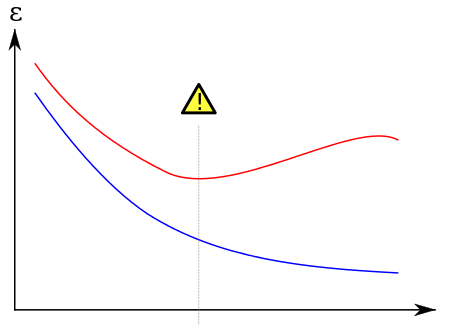
\includegraphics[width=\textwidth]{overfitting.png}

Training error: blue; validation error: red, both as a function of the number of training cycles. The best predictive and fitted model would be where the validation error has its global minimum.

\textit{Underfitting}: It occurs when the model or algorithm does not fit the data enough. It could be a bad model (too simple, or just not the right fit), or a lack of training, etc.

\textit{Classification v Regression}: A classification model is one which attempts to predict a class, or category. That is, it's predicting from a number of discrete possibilities, such as "dog" or "cat." A regression model is one which attempts to predict one or more numeric quantities, such as a temperature or a location. Which one we use depends on the nature of the variables.

\textit{Cross Validation}: The goal of cross-validation is to test the model's ability to predict new data that was not used in estimating it, in order to flag problems like overfitting or selection bias, and to give an insight on how the model will generalize to an independent dataset.

Why a CNN? It's the current state-of-the-art approach to creating computer vision models.

\section{High Level View}
Deep Learning is a Machine Learning area. The latter can be associated with the image, where update maps to learning in human terms, and more data maps to more experience (in human life). A program that learns from experience.

\begin{figure}
 \centering
 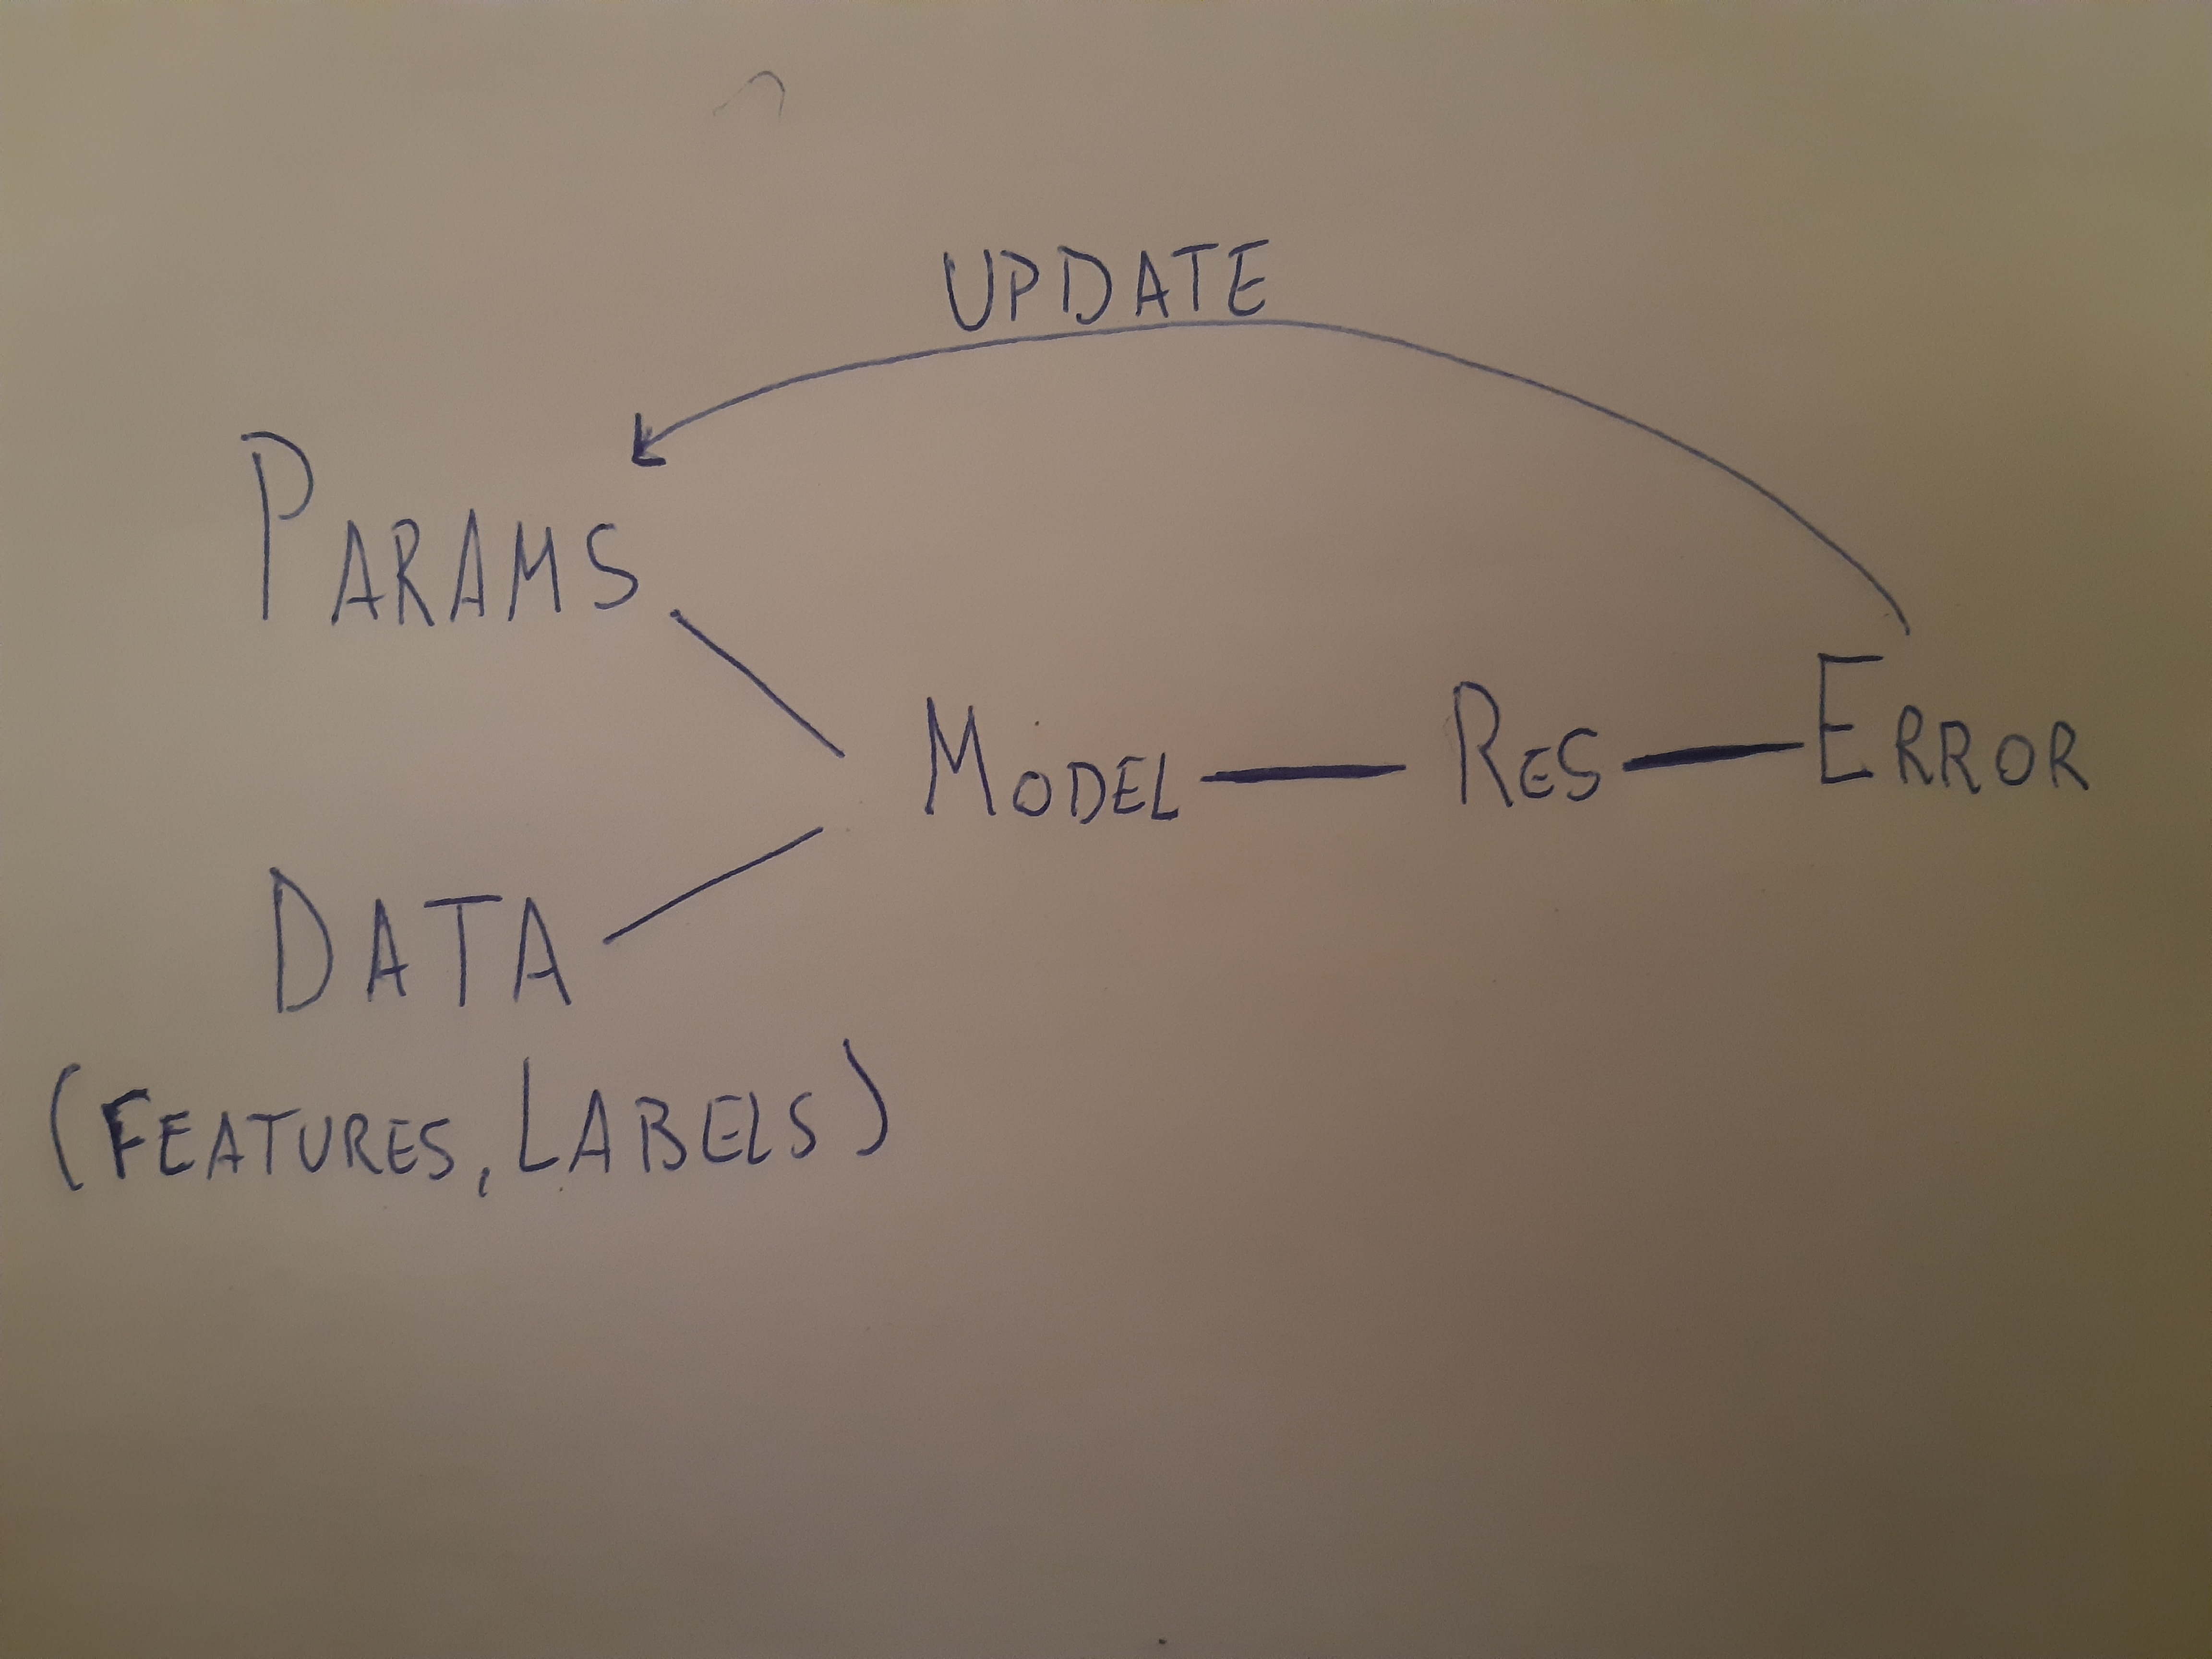
\includegraphics[width=0.9\textwidth]{ML.jpg}
 \caption{Machine Learning Process}
\end{figure}


\begin{figure}
 \centering
 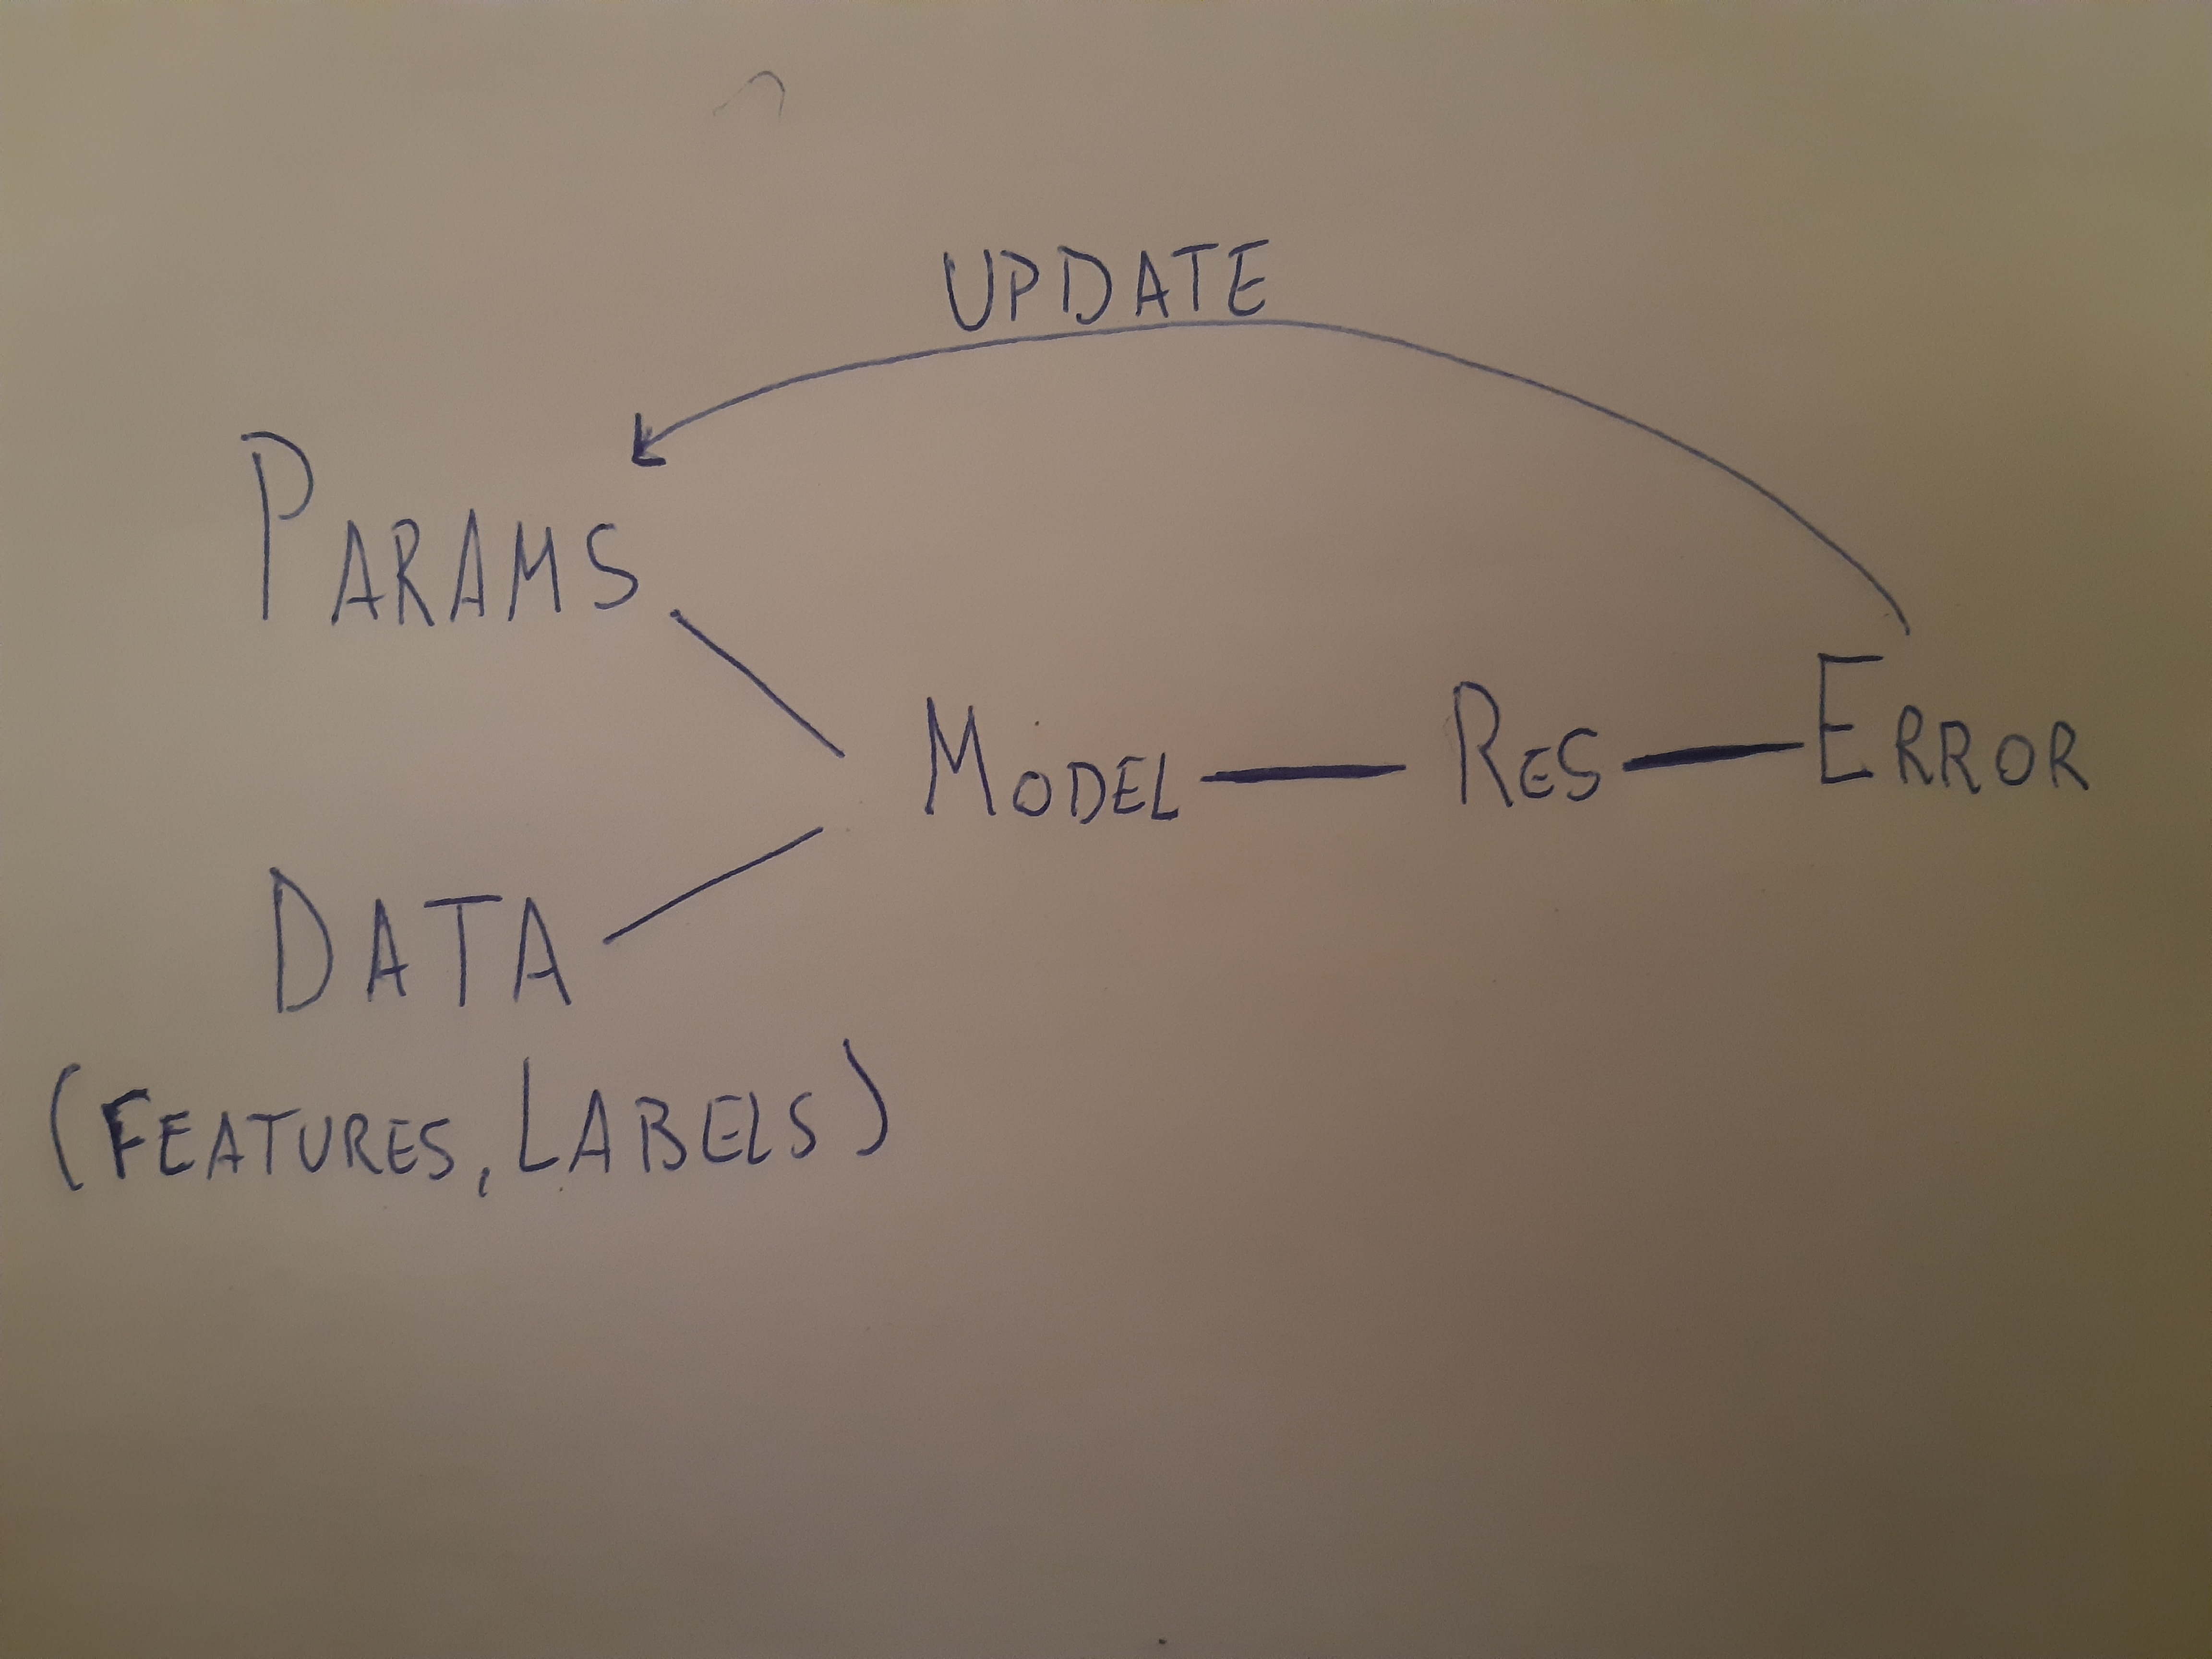
\includegraphics[width=0.9\textwidth]{ML.jpg}
 \caption{Two Layer NN}
\end{figure}


\section{Math: Basic intuitions}
Matrices are a rectangles of elements. Hence they have width and height (dimensions).

They come up as a handy notation for sets of equations (no need if there is just one equation). 

\subsection{Examples}
\textbf{One equation, one Variable}
We are told that the relation mass of flour (kilograms) to volume (in litres) of water for a particular recipe is: $$f = 2\,w + 3$$
The change or derivative is $$\frac{df}{dw} = 2x$$

\textbf{One equation, many variables}
Let's create an example where the weight of flour is always double the volume of water, $\frac{1}{5}$ of sunflower oil, and $0.01$ potasium carbonate. 

$$f(w,so,k) = 2\,w + \frac{1}{5}\,so + 0.01\,k$$

Now $f$ depends on many ingredients, instead of $f(w)$ we have $f(w,so,k,\ldots)$. In standard notation this is $f(x,y,z,\ldots)$. 

The derivative has to contemplate each variable,

\begin{align*}
  \nabla f(w,so,k) &= \frac{df}{dw} + \frac{df}{dso} \frac{df}{dk}\\
&=2 + \frac{1}{5} + 0.01
\end{align*}
Now $df$ is normally written $\nabla f$ but it means the same, derivatives respect to each component. Adding up we get a total change $df$, but a different view is keeping them separate, and hence the information on each direction (axis) isn't loose.

\begin{align*}
\nabla f(w,so,k) =
\begin{bmatrix}
   \frac{df}{dw} \\ \frac{df}{dso} \\ \frac{df}{dk}
\end{bmatrix}
=
\begin{bmatrix}
  2 \\ \frac{1}{5} \\ 0.01
\end{bmatrix}
\end{align*}

This is part of \textit{multivariate calculus} needed for DL.

\begin{center}
\begin{tabular}{cc}
  $df(x)$ & $\nabla f(x,y,z,\ldots)$\\
  $\frac{df}{dx}$ & $\frac{\partial f}{\partial x}+\frac{\partial f}{\partial z}+\ldots$
\end{tabular}
\end{center}

It was shown how many variables naturally lead to vectors - this is, they can be arranged as vectors.

\textbf{Many equations, one variable}

What happens with many equations? 

A thousand recipes containing Flour and Water in different proportions is needed for a dinner. There are $1000$ equations similar to the one above $f= k\,w + b$. $k$, $c$ being constants. $w$ could very well be a single pixel of an image. 

This can be represented as a matrix:
\begin{align*}
\begin{bmatrix}
f_1\\
f_2\\
\vdots\\
  f_{1000}
\end{bmatrix}
=
\begin{bmatrix}
k_1 & 0 & \hdots & 0_n \\
0 & k_2 & \hdots & 0_n \\
\vdots & & \hdots & \vdots \\
  0 & 0 & 0 & k_{1000}
\end{bmatrix}
\begin{bmatrix}
W_1\\
W_2\\
\vdots\\
  W_{1000}
\end{bmatrix}
+
\begin{bmatrix}
b_1\\
b_2\\
\vdots\\
  b_{1000}
\end{bmatrix}
\end{align*}

What would mean to find $d\mathbf{F}$? The equation $i^{th}$ is $f_i(w_i) = w_i\,k_i + b_i$, then $df_i = \frac{df_i}{dw_i} = k_i$ (and terms different from $i$ are $0$). $$d\mathbf{F} = \mathbf{k}$$.

What would happen if each $f_i$ is in a exponent, for example? $f_i(w_i) =  e^{w_i\,k_i + b_i}$. How are the $1000$ equations represented? Just $e^\mathbf{F}$ would indicate that. What is the derivative?

\begin{equation*}\frac{df}{dw} = e^{w_i\,k_i + b_i}\, k_i\end{equation*}. Then $$\frac{d\mathbf{F}}{dW}= \mathbf{k} \, e^\mathbf{F}$$

  In this way many derivatives can be found. For example $d\mathbf{x}^T\mathbf{x} = 2 \mathbf{x}$. Because $\mathbf{x}^T\mathbf{x}$ is a representation of a set of equations of this kind: $x^2$. A \href{https://www.gatsby.ucl.ac.uk/teaching/courses/sntn/sntn-2017/resources/Matrix_derivatives_cribsheet.pdf}{list of useful derivatives}.

For many variables, the matrix $\mathbf{k}$ has numbers other than $0$.

\chapter{Figures}

\section{Figures}\label{section:figs}
\begin{figure}[h]
 \centering
 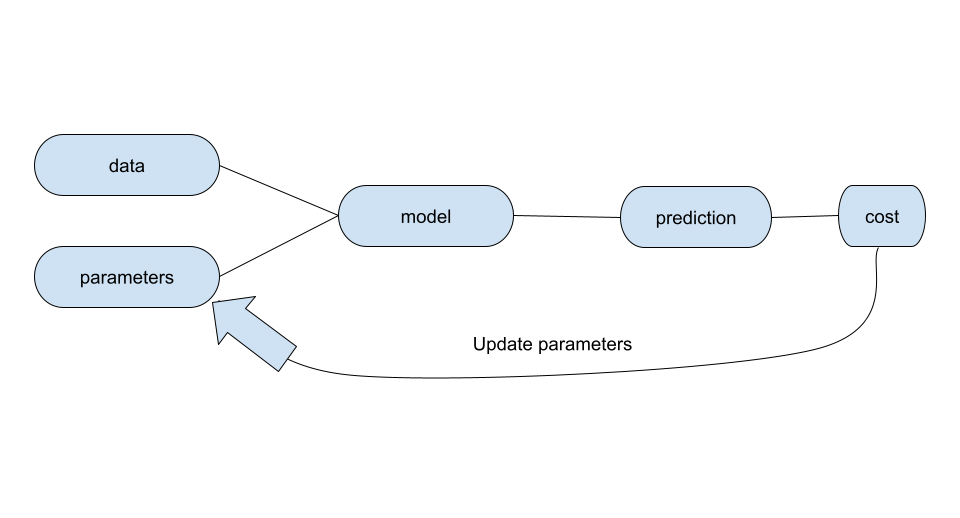
\includegraphics[width=0.9\textwidth]{ml.png}
  \caption{Machine Learning Process}\label{fig:learn}
\end{figure}

\begin{figure}
 \centering
 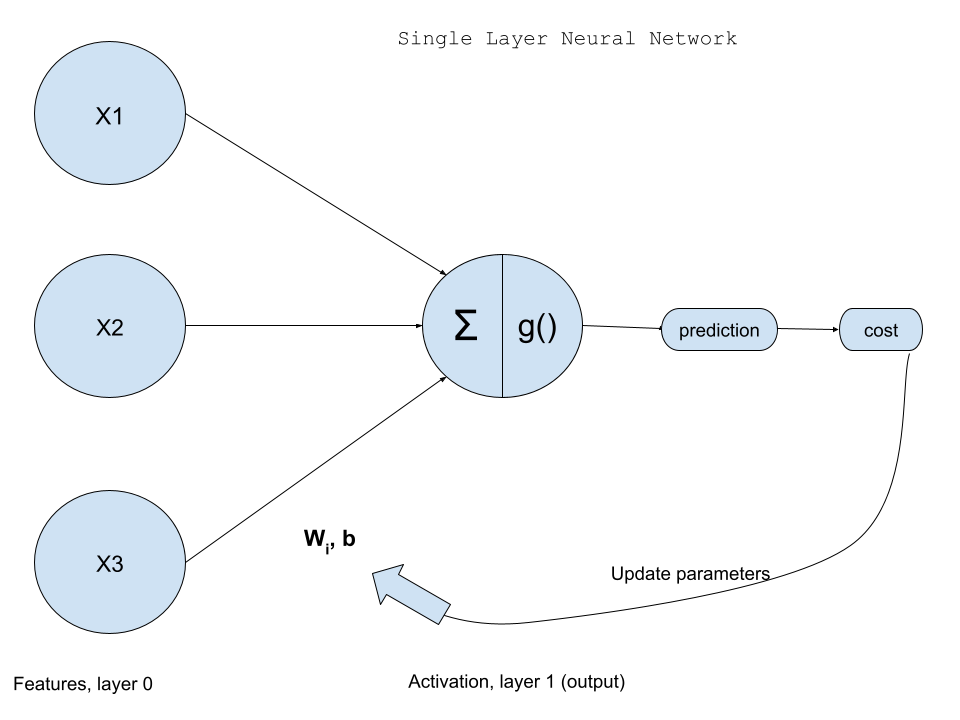
\includegraphics[width=\textwidth]{1L-NN.png}
 \caption{Single Layer Neural Network}
 \label{fig:single}
\end{figure}

\begin{figure}
 \centering
 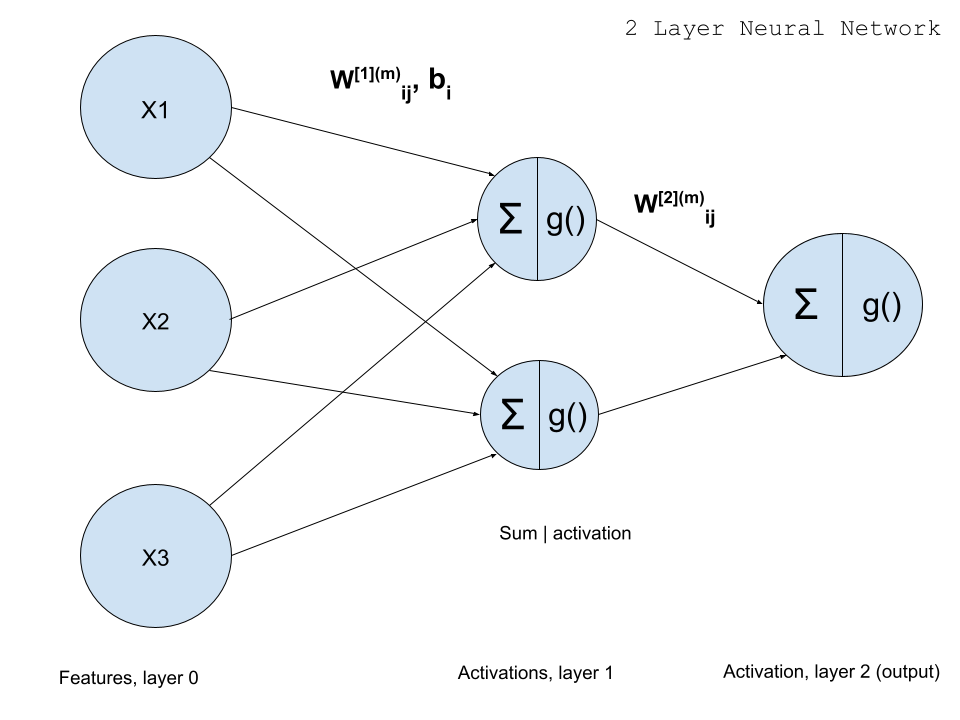
\includegraphics[width=\textwidth]{2L-NN.png}
 \caption{Shallow Neural Network}
 \label{fig:shallow}
\end{figure}

\end{document}
